\section{GPU aR-tree}

Operations on an R-tree on the GPU are expected to be memory bound. When performing ranked queries and ranked joins using R-trees with priority queue based algorithms, the access patterns are expected to be somewhat random as the R-trees are traversed in order of score. Therefore, if priority queue based algorithms are to be performed on the GPU, special care is required to achieve good random read performance when reading R-tree data from memory. Specifically, the reads should be aligned with the cache lines and memory transactions of the GPU.

The R-tree is stored as a single array of node records, containing all the records of both inner nodes and leaf nodes. The array is divided into \(h\) segments, each corresponding to a level in the R-tree. Each segment is divided into fixed size blocks of \(r\) records, each corresponding to a node in the R-tree. The segments are laid out in descending order of level so that the first segment of the array contains records belonging to the root node, and the last segment contains leaf node records. The order of blocks within each segment is unrestricted.

\begin{figure}[h]
    \centering
    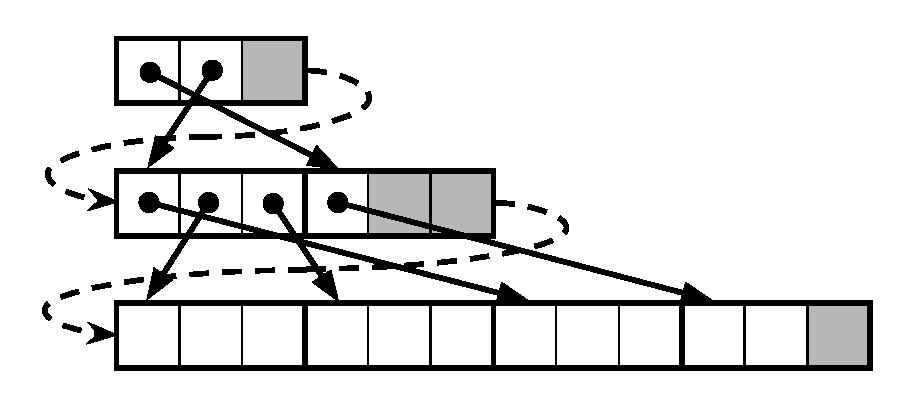
\includegraphics[scale=0.5]{memory_layout}
    \caption{R-tree memory layout with \(r = 3\).}
    \label{fig:memory-layout}
\end{figure}

Each record in the array is a \(\{mbb, score, idx\}\) tuple. For leaf node records, the \(mbb\) and \(score\) fields contain the MBB and score of an entry in the R-tree, while the remaining \(idx\) field is left unused. For inner node records, the \(mbb\) field contains the MBB of the node, and the \(score\) field contains an aggregation of the \(score\) of its children. The \(idx\) field contains the position of the block in the array that contains the records of the node.

Each block has a fixed size of \(r\) records. For a fully packed node, the block is full, but for non-full nodes, the rightmost records are used as padding. In practice, all blocks but the final block of a segment are fully packed. To access the MBBs and score (and child node references) of all the records of a node, all that has to be accessed is one fixed size block which will never be out of bounds for nodes that are not filled to capacity. For a sufficiently large input, the memory used by the padding should be negligible.

The R-tree memory layout is designed for storage in global memory on the GPU. While storing the R-tree in shared memory would allow much faster access, the R-trees are expected to be too large to fit in shared memory. Therefore, special attention is given to the alignment and size of the blocks of the record array. Ideally, blocks should be laid out so that they are naturally aligned with the memory transactions between the L1 cache, L2 cache and global memory. This allows efficiently fetching all records of a node.

\section{GPU aR-tree bulk loading}

A key element of the performance of the Depth-First Algorithm and the Block-based Algorithm is bulk loading. The Block-based algorithm performs a number of small bulk loads, and the Depth-First Algorithm performs two large bulk loads (assuming the R-trees have not been constructed prior to performing the join). To experiment with performing these algorithms on the GPU, we are interested in utilizing the GPU to perform bulk loading.

It is assumed that the unindexed data resides in device memory and that the resulting R-tree data structure will also reside in device memory. If the unindexed data originates from host memory, the unindexed data first has to be transferred to device memory. The bulk loading algorithm operates entirely within device memory, and can be controlled by a program either on the GPU or the CPU.

The bulk-loading algorithm is based on Sort-Tile-Recursive and produces an aR-tree with the aforementioned layout. Using a precomputed segment layout, it allocates an array of R-tree node records and places the data as records in the bottom level segment, then builds the R-tree from the bottom up, segment by segment until it reaches the root. The algorithm is powered by radix sort, which is a sorting algorithm that is highly efficient on the GPU.

\subsection{Computed layout}

Prior to building the R-tree, a segment layout has to be computed based on the size of the input and the fanout of the R-tree. Given an input of size \(n\) and a fanout of \(r\), the Layout Algorithm returns a segmentation of an R-tree array that fits any input of size \(n\), expressed as a list of segment sizes and offsets. The layout is only a function of the size of the input and the fanout of an R-tree that is to be bulk-loaded, it is not dependent on the actual records of the R-tree. Therefore, for repeated bulk loads such as the ones used in the Block-based Algorithm, the segmentation can be memoized and re-used for multiple bulk loads.

\begin{algorithm}
  \caption{Layout Algorithm. \(n\) is the amount of entries in the R-tree, and \(r\) is the fanout of the R-tree.}
  \label{alg/layout}
  \begin{algorithmic}[1]
    \Function{Layout}{\protect\(n, r\protect\)}
      \State{Initialize L as list of \(\lceil log_r(n) \rceil\) elements}
      \State \(i \gets 0\)
      \Repeat
        \State \(n \gets \lceil \frac{n}{r} \rceil\)
        \State \(L_i.\mathrm{size} \gets n \times r\)
        \State \(i \gets i + 1\)
      \Until{\(n \leq 1\)}
      \State \(o \gets 0\)
      \Repeat
        \State \(i \gets i - 1\)
        \State \(L_i.\mathrm{offset} \gets o\)
        \State \(o \gets o + S_i.\mathrm{size}\)
      \Until{\(i = 1\)}
      \State \Return \(L\)
    \EndFunction
  \end{algorithmic}
\end{algorithm}

The intuitive explanation for the Layout Algorithm is that \(n\) R-tree node records must be distributed into at least \(\left\lceil \frac{n}{r} \right\rceil\) nodes of size \(r\). By bulk loading \(n\) R-tree entries, \(n\) leaf node records must be distributed into at least \(\left\lceil \frac{n}{r} \right\rceil\) leaf nodes. Each leaf node will have to be placed as record in an inner node, so the process is repeated for a smaller set of \(\lceil \frac{n}{r} \rceil\) records. When the process encounters \(n \leq r\), the records can only be placed in a single node, which will become the root node.

In the basic case of \(n \leq r\), the R-tree will only be a root, and the algorithm returns the layout of a single segment for the root with a size of \(r\) and an offset of zero. When \(n > r\), the algorithm returns a layout of multiple segments. Each segment must be offset by the cumulative size of the segments of the above levels. Because \(L_1\) will lay out the last segment of the array, the total size of the array can be computed as \(L_1.\mathrm{offset} + \ L_1.\mathrm{size}\).

\subsection{Tile Partition Algorithm}

The Tile Partition Algorithm takes a segment of an R-tree record array \(S\) and partitions the records of \(S\) it into groups of size \(r\) called tiles. The algorithm is used to arrange the node records in a segment of the R-tree record array into blocks with minimal overlap.

\begin{figure}[h]
    \centering
    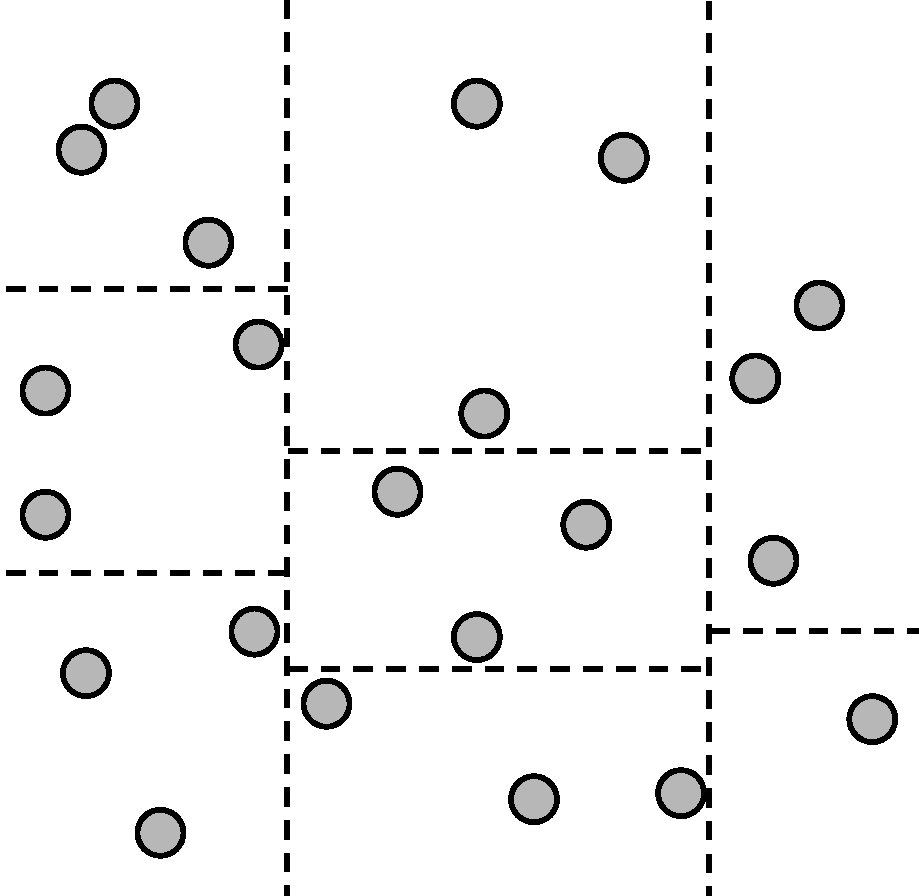
\includegraphics[scale=0.5]{sort_tile_recursive}
    \caption{Tile partitioning of 22 records for \(r = 3\), first sorted by \(x\) coordinate (left to right) then \(y\) coordinate (top to bottom).}
    \label{fig:sort-tile-recursive}
\end{figure}

The algorithm relies on a segmented sorting algorithm. Given an array of keys \(K\), an array of values \(S\) and a segment size of \(s\), the segmented sorting algorithm divides the input into \(k\) segments of size \(s\) \(K_0, K_1, \dotsc, K_{k - 1}\) and \(S_0, S_1, \dotsc, S_{k - 1}\), then sorts each pair \((K_i, S_i)\) independently. The sorting operation sorts the values by their associated keys. Segmented sorting can be parallelized using radix sort on the GPU.

\begin{algorithm}
  \caption{Tile Partition Algorithm. \(S\) is a segment of the R-tree record array, \(r\) is the block size, and \(d\) is the number of dimensions.}
  \label{alg/tile-partition}
  \begin{algorithmic}[1]
    \Function{GpuTilePartition}{\protect\(S, r, d\protect\)}
      \State{Initialize K as list of \(|S|\) elements}
      \State{\(s \gets \left\lceil \sqrt[k]{\frac{|S|}{r}} \right\rceil\)}
      \State{\(l \gets r d^{k}\)}
      \For{\(i \gets 0, d - 1\)}
        \ForAll{\(j \in 0, 1, \dotsc, |S| - 1\) in parallel}
          \State{\(K_j \gets S_j.\mathrm{mbb}.\min_i\)}
        \EndFor
        \State{\(S \gets\) \Call{SegmentedRadixSort}{K, S, l}}
        \State{\(l \gets \frac{s}{s}\)}
      \EndFor
      \State \Return \(S\) 
    \EndFunction
  \end{algorithmic}
\end{algorithm}

The algorithm works by iteratively dividing the input into smaller segments, considering one dimension at a time. In the two-dimensional case, the algorithm first divides the input into vertical slices, then it divides each slice into tiles (blocks). In the three-dimensional case, the algorithm first divides the input into slabs, then divides each slab into pillars, then divides each pillar into a block. \(l\) represents the current size of each segment, and is initially as large as the input segment. \(s\) represents the amount of segments each segment can be divided into, leading to a total of \(s^k\) groups, which has to satisfy the requirement \(r s^k \geq |S|\). If \(|S|\) is not divisible by \(r d^k\), the final segment may contain fewer records than the others.

\subsection{Tile Build Algorithm}

After partitioning of the R-tree node records of a level \(i\), the records of level \(i + 1\) can be produced. The Tile Build Algorithm takes an input segment of R-tree node records and returns an output segment of inner node records. It calculates and records the aggregate score and the MBBs of the inner node records. The score aggregation is MAX, which creates upper bounds.

\begin{algorithm}
  \caption{Tile Build Algorithm. \(S\) is a segment of the R-tree record array and \(r\) is the block size.}
  \label{alg/tile-build}
  \begin{algorithmic}[1]
    \Function{GpuTileBuild}{\protect\(S, r\protect\)}
      \State Initialize \(O\) as list of \(\lceil |S| / r \rceil\) elements
      \ForAll{\(i \in 0, 1, \dotsc, \lceil |S| / r \rceil - 1\) in parallel}
        \State{\(j \gets ir\)}
        \State{\(k \gets\) \Call{Min}{\protect\(j + r, |S|\protect\)}}
        \State{\(O_i.\mathrm{mbb} \gets\) \Call{Reduce}{Mbb, \protect\(\{S_j.\mathrm{mbb}, S_{j + 1}.\mathrm{mbb}, \dotsc, S_{k - 1}.\mathrm{mbb} \}\protect\)}}
        \State{\(O_i.\mathrm{score} \gets\) \Call{Reduce}{MAX, \protect\(\{S_j.\mathrm{score}, S_{j + 1}.\mathrm{score}, \dotsc, S_{k - 1}.\mathrm{score}\}\protect\)}}
        \State{\(O_i.\mathrm{idx} \gets j\)}
      \EndFor
      \State \Return \(O\)
    \EndFunction
  \end{algorithmic}
\end{algorithm}

A key detail is that the Tile Build Algorithm is not limited to parallelization per output element. In fact, it can be efficiently parallelized with a thread per input element. On GPU, the evaluation of each MBB and score MAX value in the output can be evaluated using parallel reduce operations.

\subsection{STR}

Finally, the full Sort-Tile-Recursive algorithm can be described in full. Given an input \(I\) of \(n\) elements, each with a score and an MBB, it returns an array of R-tree records according to the layout \(L\) that contains the input elements. First, the STR algorithm places the input data as leaf node records in the final segment of the array of R-tree records. Then for all but the last level (the root level), the algorithm first partitions the node records of the current level into tiles, then builds the next level of node records. The last level is guaranteed to consist of only the root node and is of size \(r\), therefore it requires no sorting, nor has any level above it to be built. The resulting array contains all segments in descending order of level.

\begin{algorithm}
  \caption{STR. \(L\) is the layout of the R-tree, \(I\) is a list of entries to be inserted, \(r\) is the block size and \(d\) is the number of dimensions.}
  \label{alg/str}
  \begin{algorithmic}[1]
    \Function{GpuStr}{\protect\(L, I, r, d\protect\)}
      \State Initialize \(R\) as list of \(L_0.\mathrm{offset} + L_0.\mathrm{size}\) elements
      %\State Initialize \(S\) as list of \(h\) elements
      \ForAll{\(i \in 0, 1, \dotsc, n - 1\) in parallel}
        \State \(R_{L_0.\mathrm{offset} + i}.\mathrm{mbb} = I_i.\mathrm{mbb}\)
        \State \(R_{L_0.\mathrm{offset} + i}.\mathrm{score} = I_i.\mathrm{score}\)
      \EndFor
      \For{\(i \gets 0,\, |L| - 1\)}
        \State \(j_0 \gets L_i.\mathrm{offset}\)
        \State \(k_0 \gets j_0 + L_i.\mathrm{size} - 1\)
        \State \(j_1 \gets L_{i + 1}.\mathrm{offset}\)
        \State \(k_1 \gets j_1 + L_{i + 1}.\mathrm{size} - 1\)
        \State \(R_{j_0, j_0 + 1, \dotsc, k_0} \gets\) \Call{GpuTilePartition}{\protect\(R_{j_0, j_0 + 1, \dotsc, k_0}, r, d\protect\)}
        \State \(R_{j_1, j_1 + 1, \dotsc, k_1} \gets\) \Call{GpuTileBuild}{\protect\(R_{j_0, j_0 + 1, \dotsc, k_0}, r\protect\)}
      \EndFor
      \State \Return \(R\)
    \EndFunction
  \end{algorithmic}
\end{algorithm}

\section{GPU top-k R-tree join}

The GPU Ranked R-tree Join Algorithm is based on the work of Qi et al.~\cite{qi2013efficient}. Given two aR-trees \(A\) and \(B\), it returns the top-\(k\) joined elements above the score threshold \(\theta\). The threshold may be set to \(\theta = -\infty\), in which case the threshold is effectively ignored. The algorithm is a key part of both the Distance-First Algorithm and the Block-based Algorithm.

The algorithm operates on a priority queue implemented as a parallel heap that resides. Each element in the queue refers to two intersecting nodes, one from \(A\) and the other from \(B\). The priority queue is initialized with references to the root nodes of \(A\) and \(B\). In each pass, the top element of the queue is dequeued, then all records of the node of \(A\) and \(B\) are fetched from global memory. Then all combinations of node records are evaluated in parallel, producing anywhere from zero to \(r^2\) results which are temporarily placed into \(V\) as candidate result. \(V\) may contain a number of \(Nil\) values, so \(V\) is compacted to filter out \(Nil\) entries. If the records are inner node records, the elements of \(V\) are placed into the priority queue. If not, the elements of \(V\) are placed as candidate results into \(C\) so that \(C\) retains the current top-\(k\) elements.

The score threshold \(\theta\) is continuously updated to represent the \(k^{th}\) greatest score seen so far when candidate results are discovered. Until \(k\) candidate results are discovered, \(\theta\) remains at its initial value. When an element of the priority queue is dequeued with a score below \(\theta\), the join can no longer produce elements with a score that satisfies the score threshold, so the algorithm terminates. The algorithm will also terminate if the queue has no remaining elements.

\begin{algorithm}
  \caption{Ranked R-tree Join Algorithm. \(k\) is the amount of elements to be returned, \(A\) is the first R-tree, \(B\) is the second R-tree, \(\theta\) is the score threshold, \(\phi\) is the spatial predicate used to join the R-tree nodes and \(\gamma\) is the score aggregate function.}
  \label{alg/ranked-r-tree-join}
  \begin{algorithmic}[1]
    \Function{GpuRankedRTreeJoin}{\protect\(k, A, B, \theta, \gamma, \phi\protect\)}
      \State Initialize \(Q\) as a priority queue with initial entry \(\{ .score=0,\, .level=h - 1,\, .aIdx=0,\, .bIdx=0 \}\)
      \State Initialize \(C\) as shared list of size \(k\)
      % \State Initialize \(T\) and \(U\) as shared lists of size \(r\)
      \State Initialize \(V\) as a shared list of size \(r^2\)
      \While{\(Q\) is not empty}
        \State \(e \gets\) \Call{Dequeue}{\protect\(Q\protect\)}
        \If{\(e.\mathrm{score} < \theta\)}
          \State \Return \(C\) \Comment{No more elements with sufficient score}
        \EndIf
        % \ForAll{\(i \in 0, 1, \dotsc, r - 1\) in parallel}
        %   \State \(T_i \gets A_{e.\mathrm{aIdx} + i}\)
        %   \State \(U_i \gets B_{e.\mathrm{bIdx} + i}\)
        % \EndFor
        \ForAll{\((i, j) \in (0, 1, \dotsc, r - 1) \times (0, 1 \dotsc, r- 1)\) in parallel}
          \State \(s \gets\) \Call{\(\gamma\)}{\protect\(A_{e.\mathrm{aIdx} + i}.\mathrm{score}, B_{e.\mathrm{bIdx} + j}.\mathrm{score}\protect\)}
          \If{\Call{\(\phi\)}{\protect\(A_{e.\mathrm{aIdx} + i}.\mathrm{mbb}, B_{e.\mathrm{bIdx} + j}.\mathrm{mbb}\protect\)} and \(s \geq \theta\)}
            \State \(V_{rj + i}.\mathrm{score} \gets s\)
            \State \(V_{rj + i}.\mathrm{level} \gets e.\mathrm{level} - 1\)
            \State \(V_{rj + i}.\mathrm{aIdx} \gets A_{e.\mathrm{aIdx} + i}.\mathrm{idx}\)
            \State \(V_{rj + i}.\mathrm{bIdx} \gets B_{e.\mathrm{bIdx} + j}.\mathrm{idx}\)
          \Else
            \State \(V_{rj + i} \gets Nil\)
          \EndIf
        \EndFor
        \State \Call{Compact}{\protect\(V\protect\)}
        \If{\(e.\mathrm{level} > 0\)} \Comment{Pairs of inner node records}
          \State \Call{Enqueue}{\protect\(Q, V\protect\)}
        \Else \Comment{Pairs of leaf node records}
          \State \(C \gets\) \Call{TopK}{\protect\(C + V, k\protect\)}
          \If{\(|C| = k\)}
            \State \(\theta \gets C_{k - 1}\)
          \EndIf
        \EndIf
      \EndWhile
      \State \Return \(C\) \Comment{No more elements}
    \EndFunction
  \end{algorithmic}
\end{algorithm}

The main draw of the algorithm is that it is an implementation of a ranked R-tree join that can run on the GPU, but its performance is expected to be limited. Even though the algorithm can utilize parallelism to evaluate the spatial predicate for all combinations in parallel on the GPU, it is not expected to outperform an implementation of a ranked R-tree join on the CPU in the general case. The reason for this is that the cost of compacting, sorting and maintaining the priority queue is expected to be high. Additionally, the kernel will be spending some time waiting for the node records to be fetched from global memory. The algorithm can instead be parallelized by running multiple instances of the algorithm in parallel. The algorithm fits naturally into a thread group of size \(r^2\), so a number of thread groups can be created to allow interleaved execution multiple ranked R-tree joins.

Ideally, the parallel heap will reside in shared memory for its fast memory access characteristics, but shared memory may not be able to hold enough elements for sufficiently large values of \(k\) or large R-trees with bad score distributions. Even if the queue is small enough to fit into shared memory, it should also be sufficiently small to allow multiple thread blocks to execute on the same streaming multiprocessor. The top of the parallel heap could be placed in shared memory and the while could be placed in global memory. Alternatively, when the queue grows sufficiently large, the task could be divided into subproblems by distributing the elements of the parallel heap into additional thread groups, then concatenating their top-k results. Another strategy would be to keep the size of the R-trees sufficiently small to prevent overflow.

\section{GPU Block-based Algorithm}

Like the Block-based Algorithm, the GPU Block-based Algorithm reads the inputs in order of descending rank, one block at a time. It uses the GPU STR algorithm to bulk load R-trees from each loaded input block, then evaluates a GPU ranked R-tree join in parallel for each previously loaded block of the other input. Similar to HRJN, the aggregate score of the last accessed item of input A and the first accessed item of input B forms an upper bound for the score of any joined item produced by reading another block of A, and the aggregate score of the last accessed item of input B and the first accessed item of input A forms an upper bound for the score of any joined item produced by reading another block of B. This is used to create a threshold \(T\) for all join results that have not been produced. When the \(k^{th}\) candidate result has a score above the threshold, the candidate results of \(C\) are known to be the top-k result.

Assuming the inputs reside in host memory, the inputs have to be transferred to device memory first. Before joining, the unindexed inputs have to be sorted in descending order of score. If they are not already sorted, the sort can be performed entirely on the GPU using radix sort.

The algorithm is expected to start relatively slow due to a limited level of parallelism, but its parallelism scales as more blocks are read and bulk loaded into R-trees. Each time a block is read and bulk loaded into an R-tree, another join can be performed in parallel. The rate of increase in parallelism is dependent to the block size, which should be kept relatively low for sufficient increase in parallelism, though increasing levels of parallelism will increase the amount of work.

\begin{algorithm}
  \caption{Block-based Algorithm. \(k\) is the amount of elements to return, \(A\) and \(B\) are the spatial inputs, \(\gamma\) is the score aggregate function and \(\phi\) is the spatial predicate.}
  \label{alg/block-based}
  \begin{algorithmic}[1]
    \Function{GpuBlockTopK}{\protect\(k, A, B, \gamma, \phi\protect\)}
      \State Initialize \(C\) as list of size \(k\)
      \State Sort \(A\) and \(B\) if not already sorted
      \State \(\theta \gets -\infty\)
      \While{more blocks of objects exist in \(A\) and \(B\)}
        \State \(i \gets\) next input to be accessed \Comment{\(A\) or \(B\)}
        \State \(j \gets\) the other input \Comment{\(A\) or \(B\)}
        \State \(P \gets\) \Call{GetNextBlock}{\protect\(i\protect\)}
        \State \(L \gets\) \Call{Layout}{\protect\(|P|, r\protect\)}
        \State \(R_P \gets\) \Call{GpuStr}{\protect\(L, P, r, \gamma_l, k\protect\)}
        \State Initialize \(V\) as list
        \ForAll{blocks \(P'\) of \(j\) in parallel}
          \State \(V \gets V +\) \Call{GpuRankedRTreeJoin}{\protect\(k, R_P, {R_P}', \theta, \gamma_r, \phi\protect\)}
        \EndFor
        \State \(C \gets\) \Call{TopK}{\protect\(k, C + V\protect\)}
        \If{\(|C| = k\)}
          \State \(\theta \gets C_{k - 1}\)
        \EndIf
        \State \(T \gets \mathrm{MAX}(\gamma(A_{first}.\mathrm{score}, B_{last}.\mathrm{score}), \gamma(A_{last}.\mathrm{score}, B_{first}.\mathrm{score}))\)
        \If{\(T < \theta\)}
          \State \Return \(C\) \Comment{No more elements with sufficient score}
        \EndIf
      \EndWhile
      \State \Return \(C\) \Comment{No more input elements}
    \EndFunction
  \end{algorithmic}
\end{algorithm}
